\chapter{需求建模}
\section{数据流图}
\subsection{顶层数据流图}
\subsection{0层数据流图}
\begin{figure}[H]
\centering
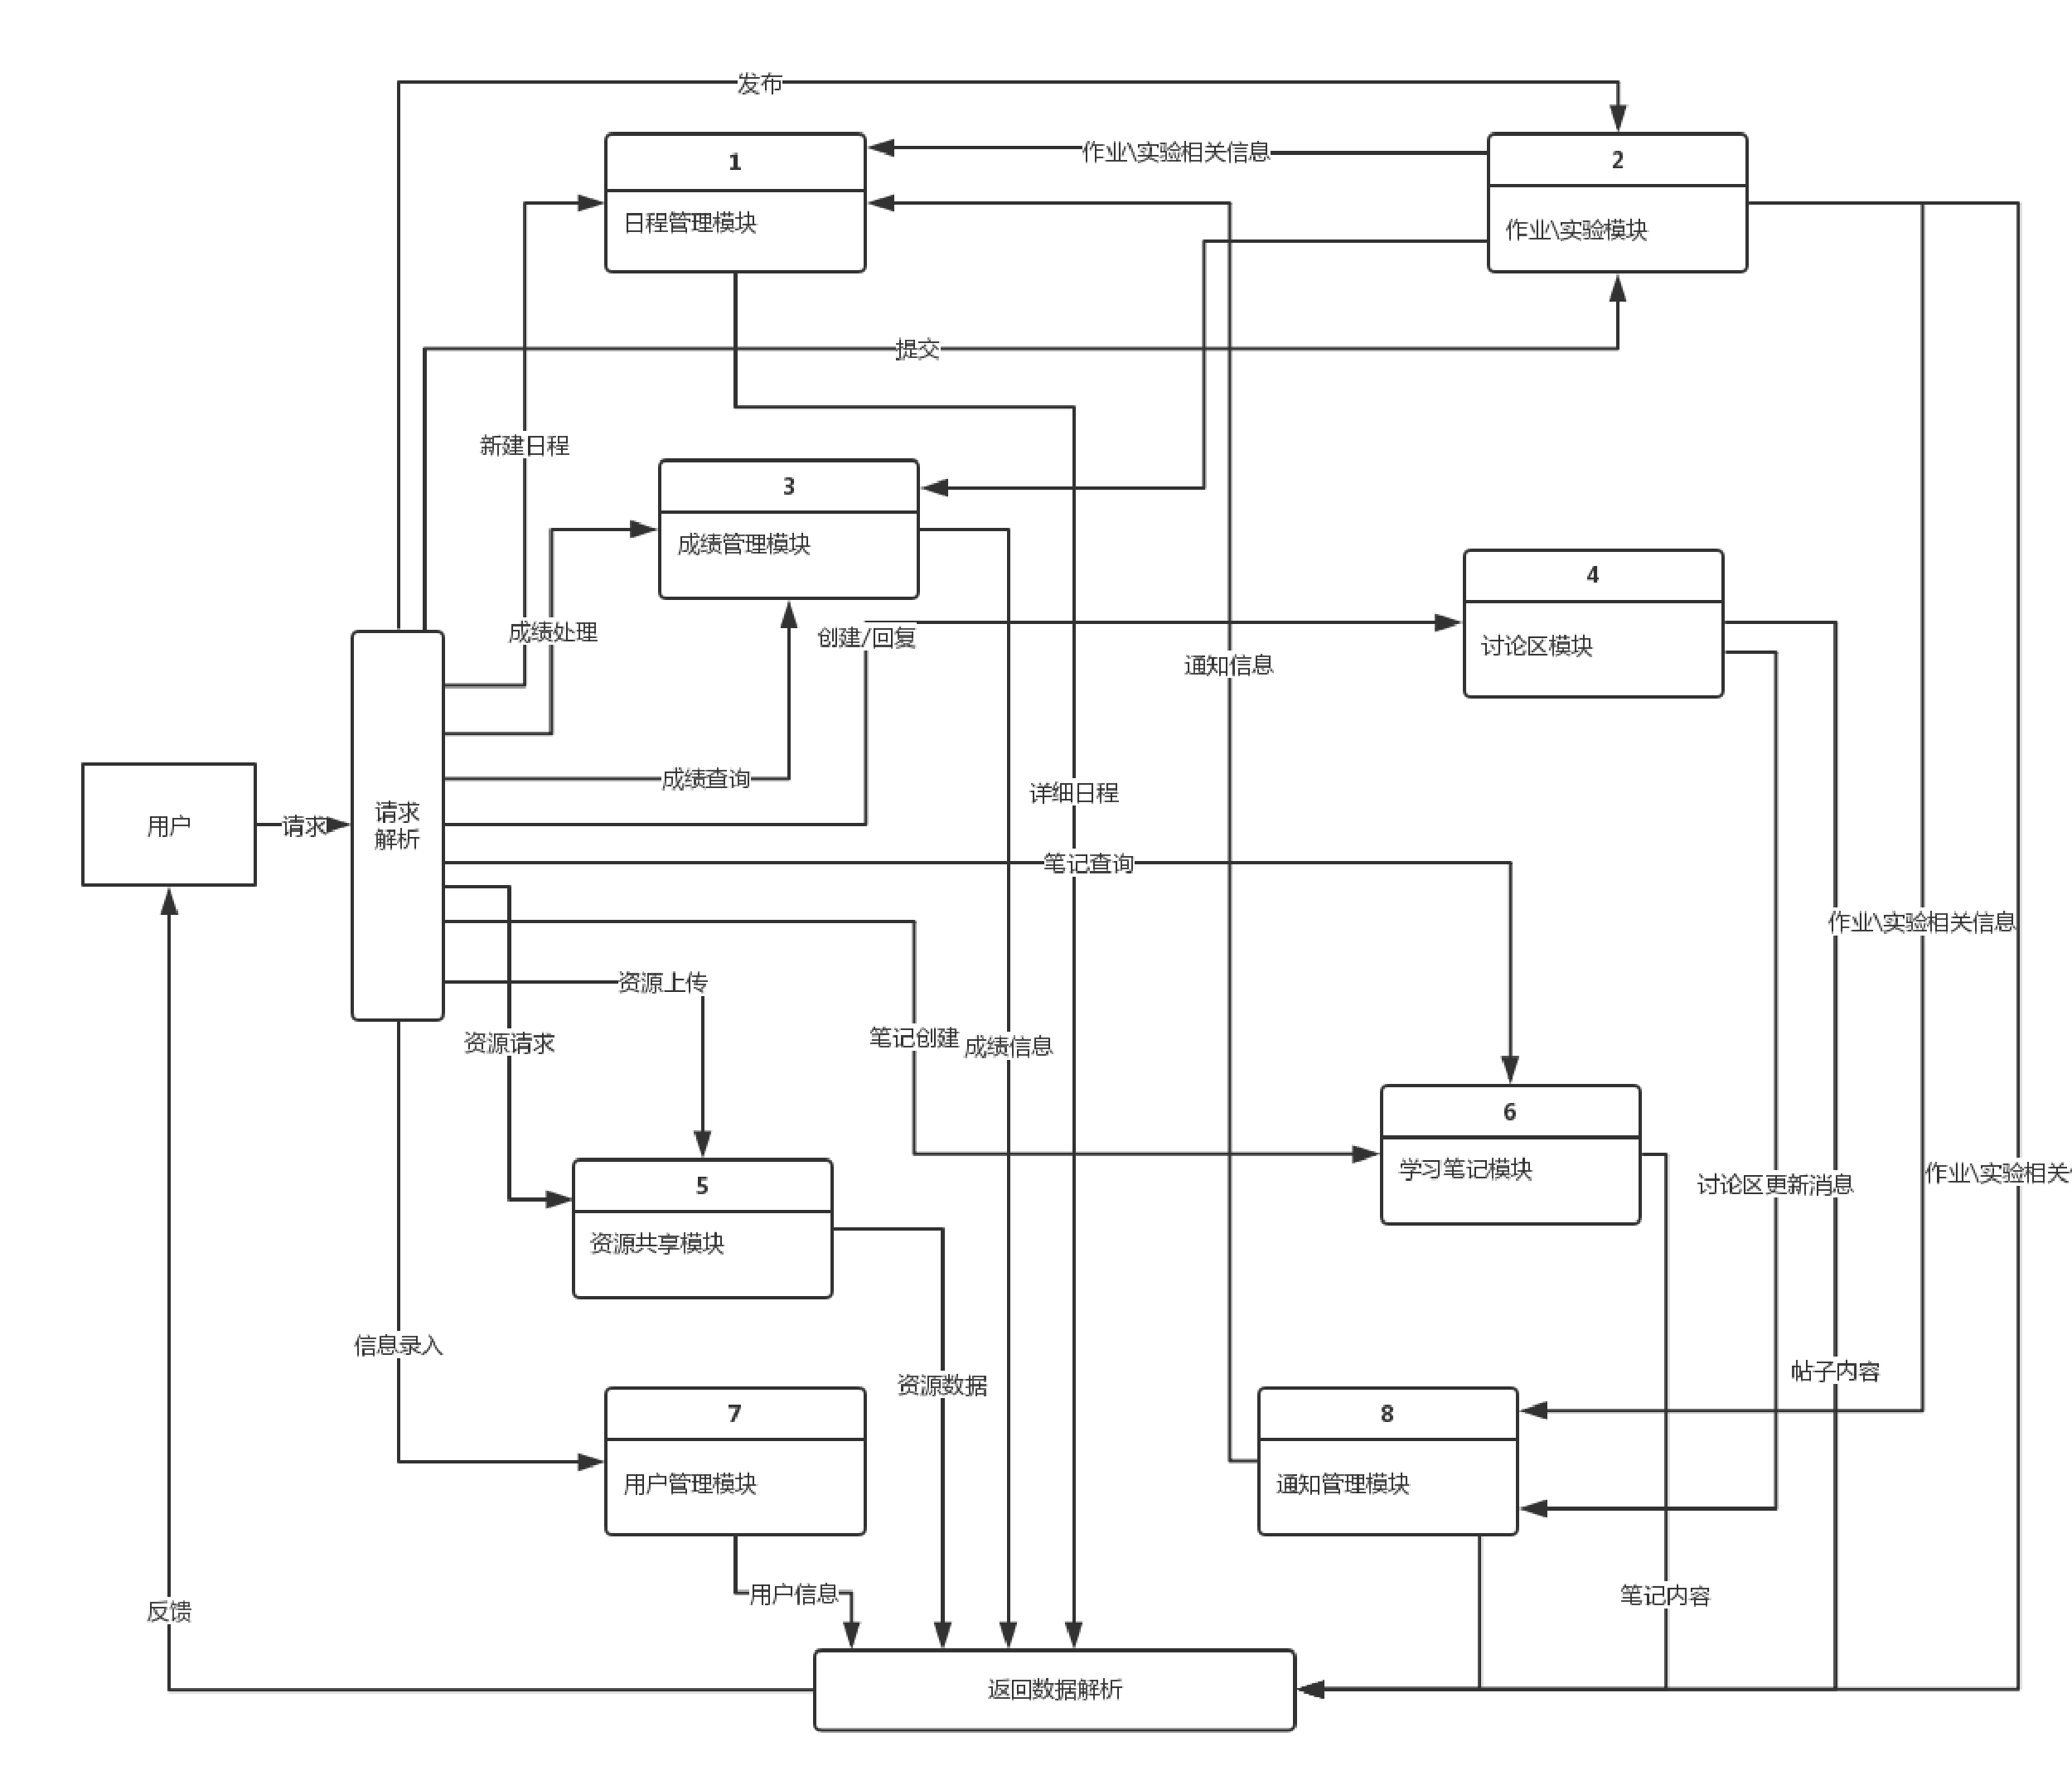
\includegraphics[width=18cm]{Level_0}
\caption{0层数据流图}
\end{figure}
\subsection{1层数据流图}
\subsubsection{日程管理模块}
\begin{figure}[H]
\centering
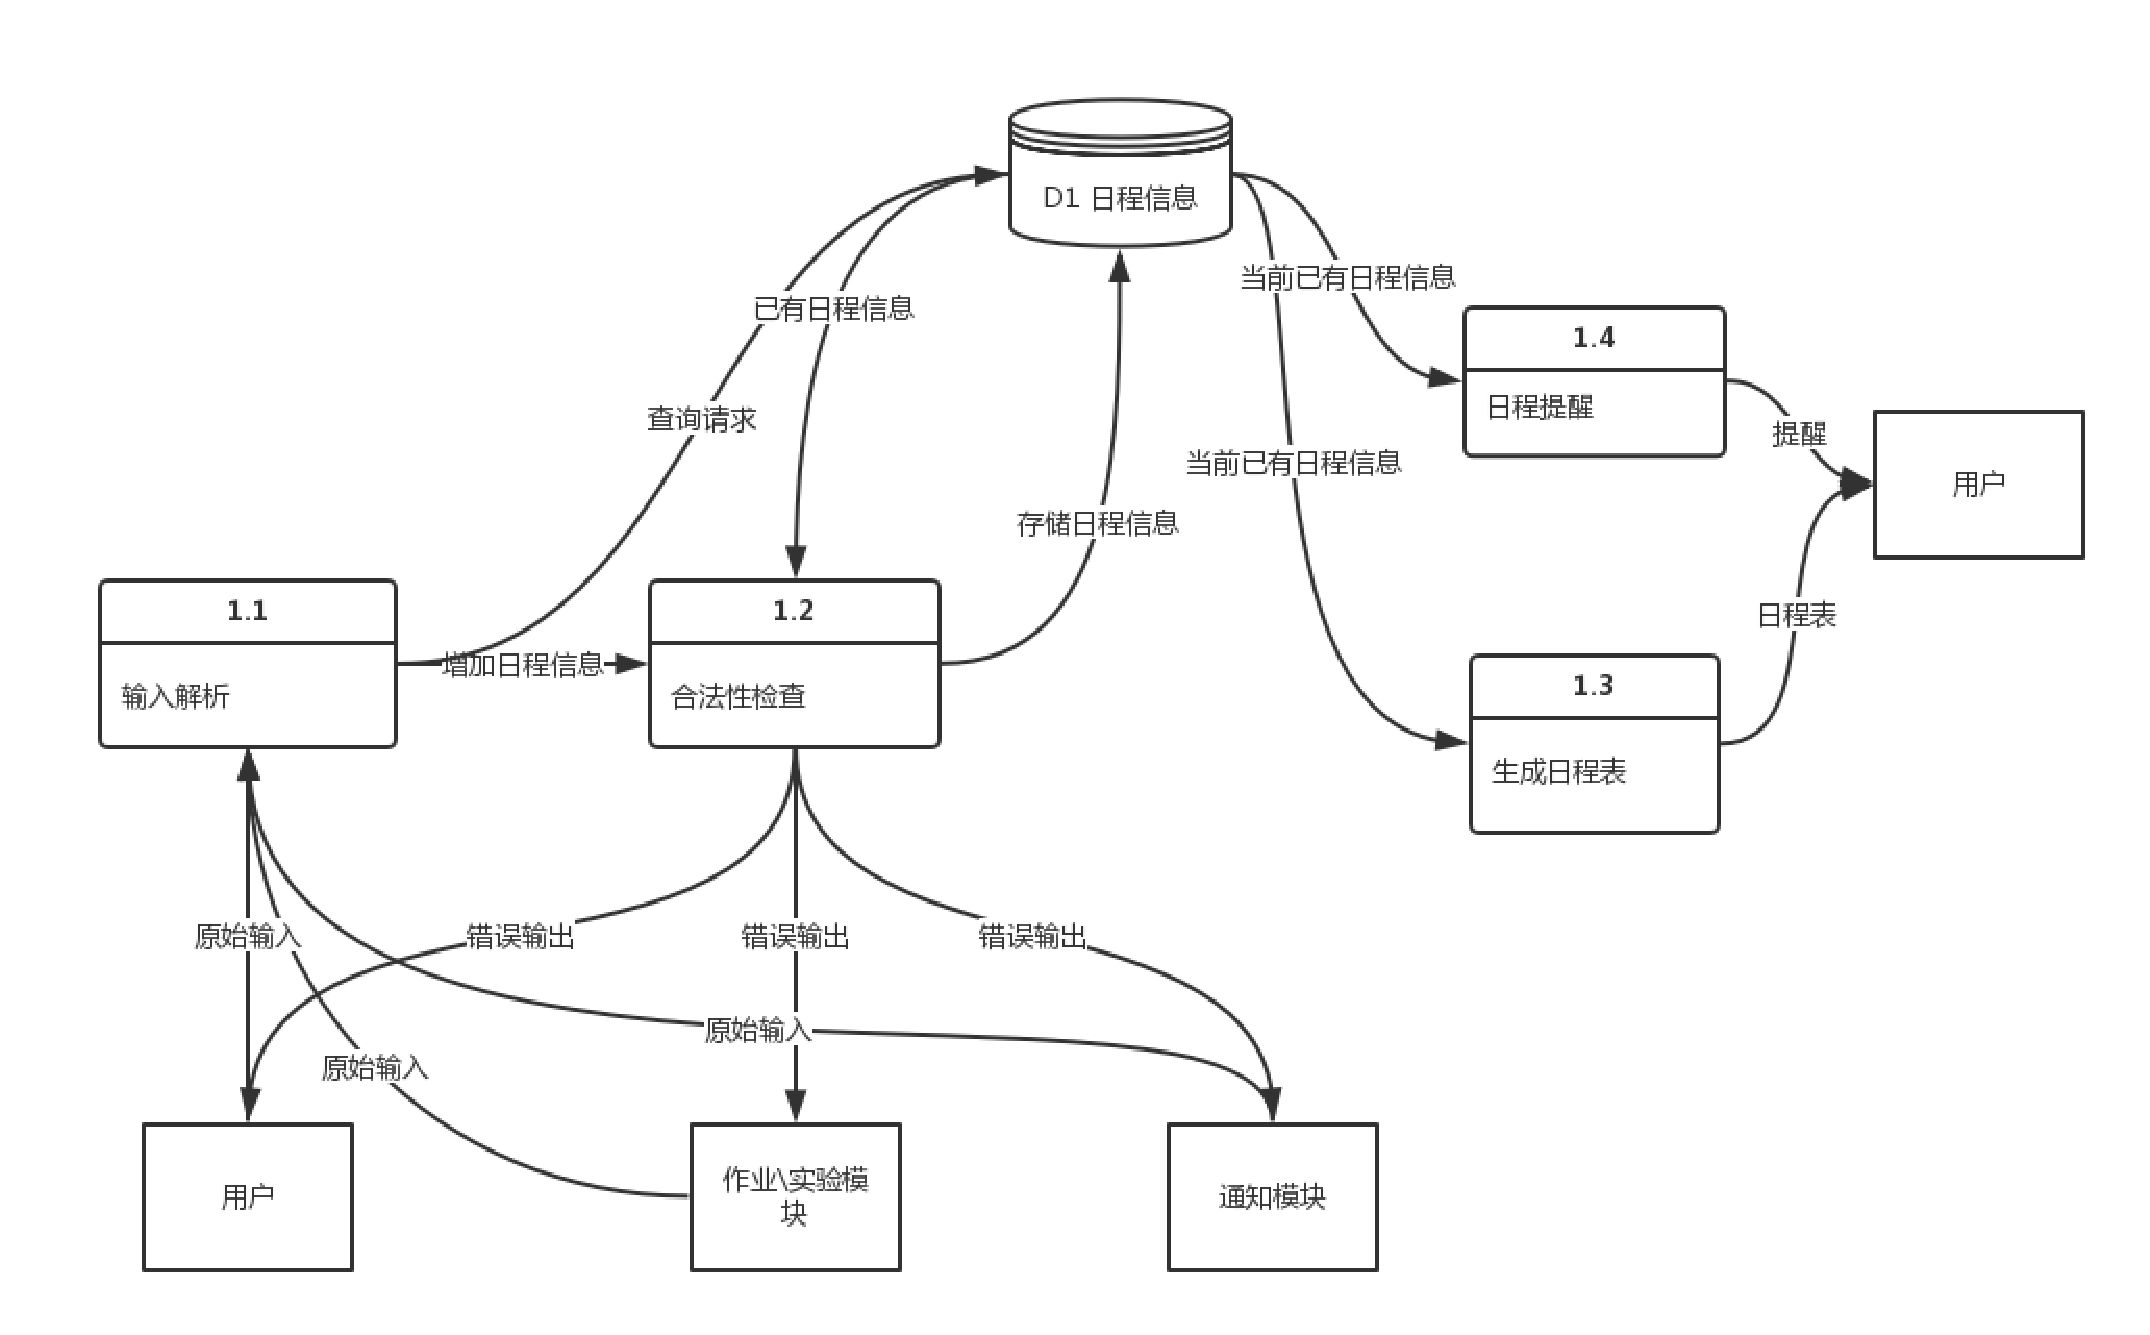
\includegraphics[width=15cm]{level1_日程管理}
\caption{日程管理模块功能数据流图}
\end{figure}
\subsubsection{作业实验模块}
\begin{figure}[H]
\centering
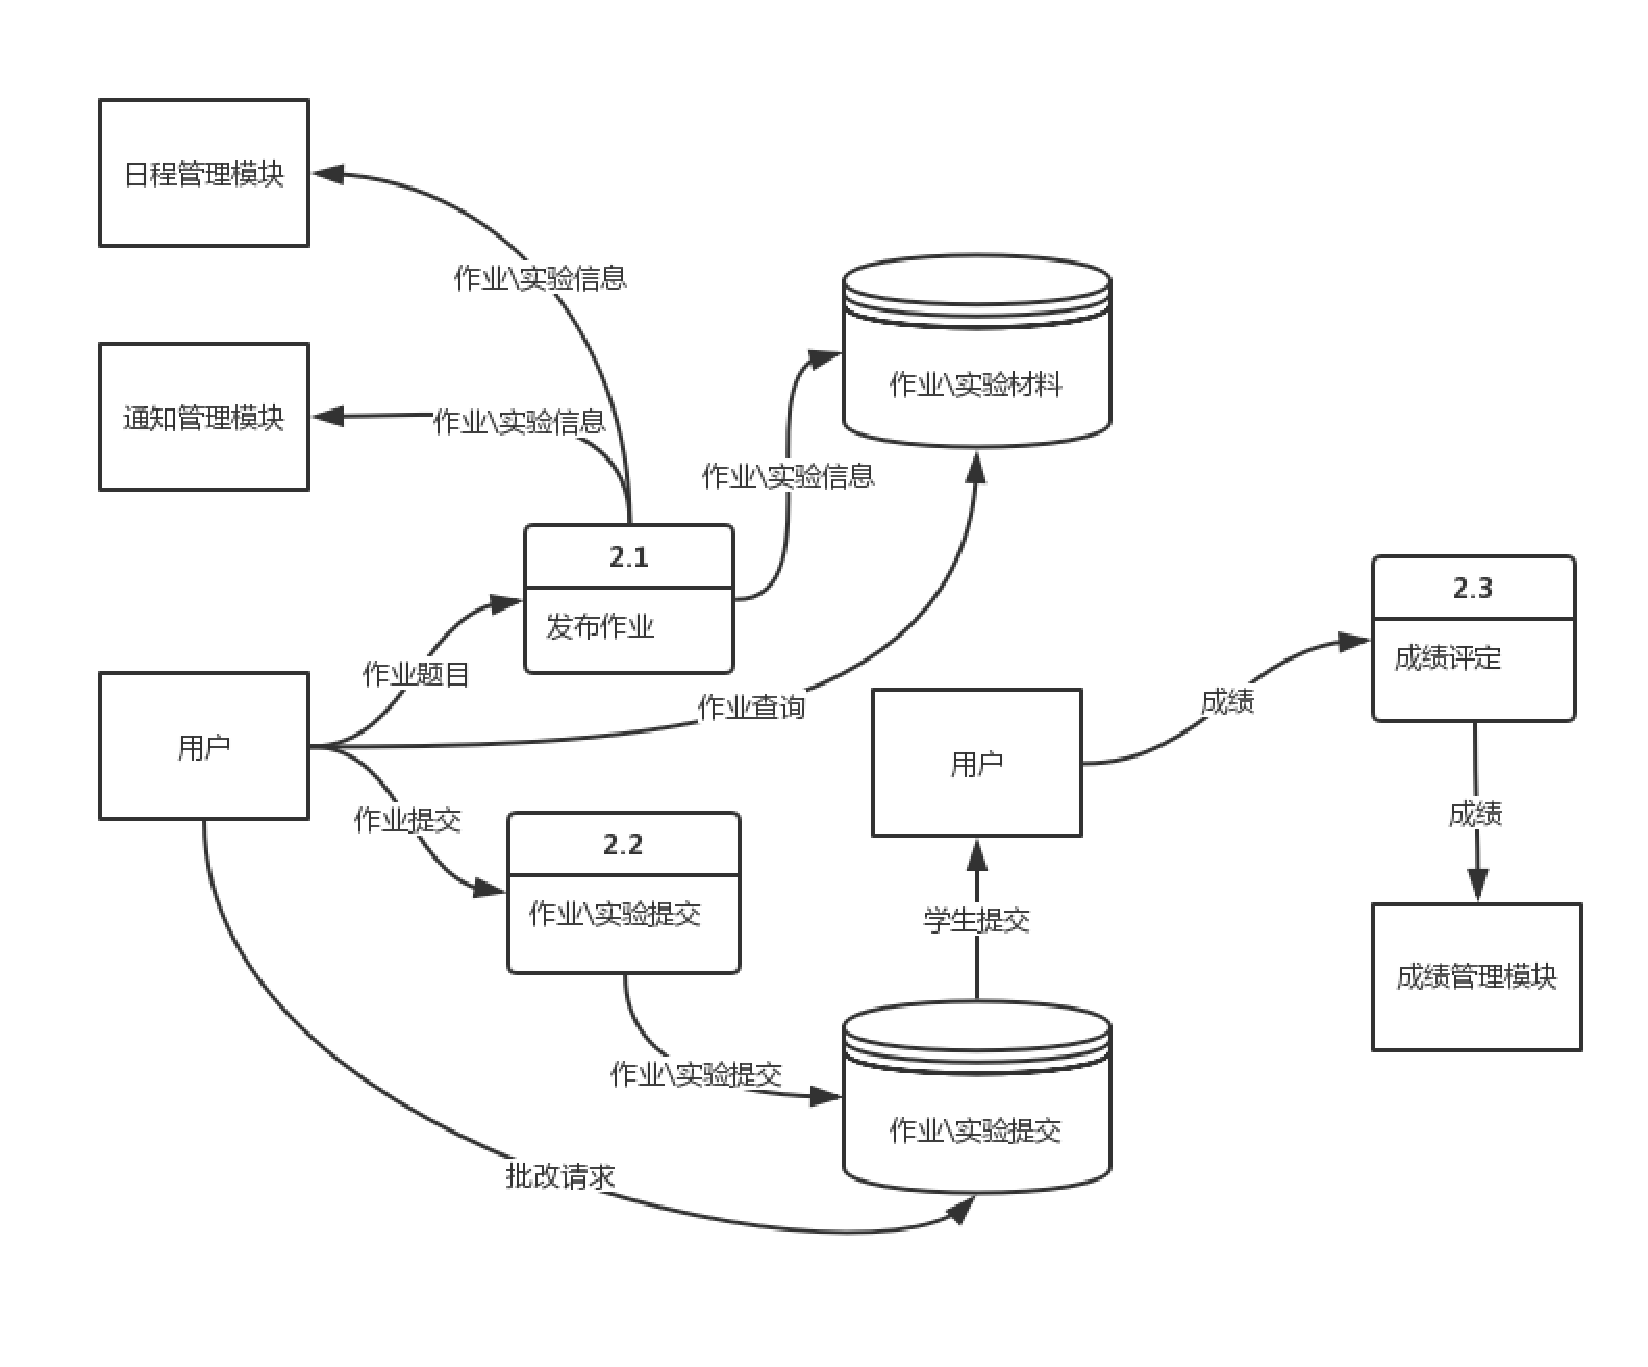
\includegraphics[width=15cm]{level1_作业}
\caption{日程管理模块功能数据流图}
\end{figure}
\subsubsection{学习笔记模块}
\begin{figure}[H]
\centering
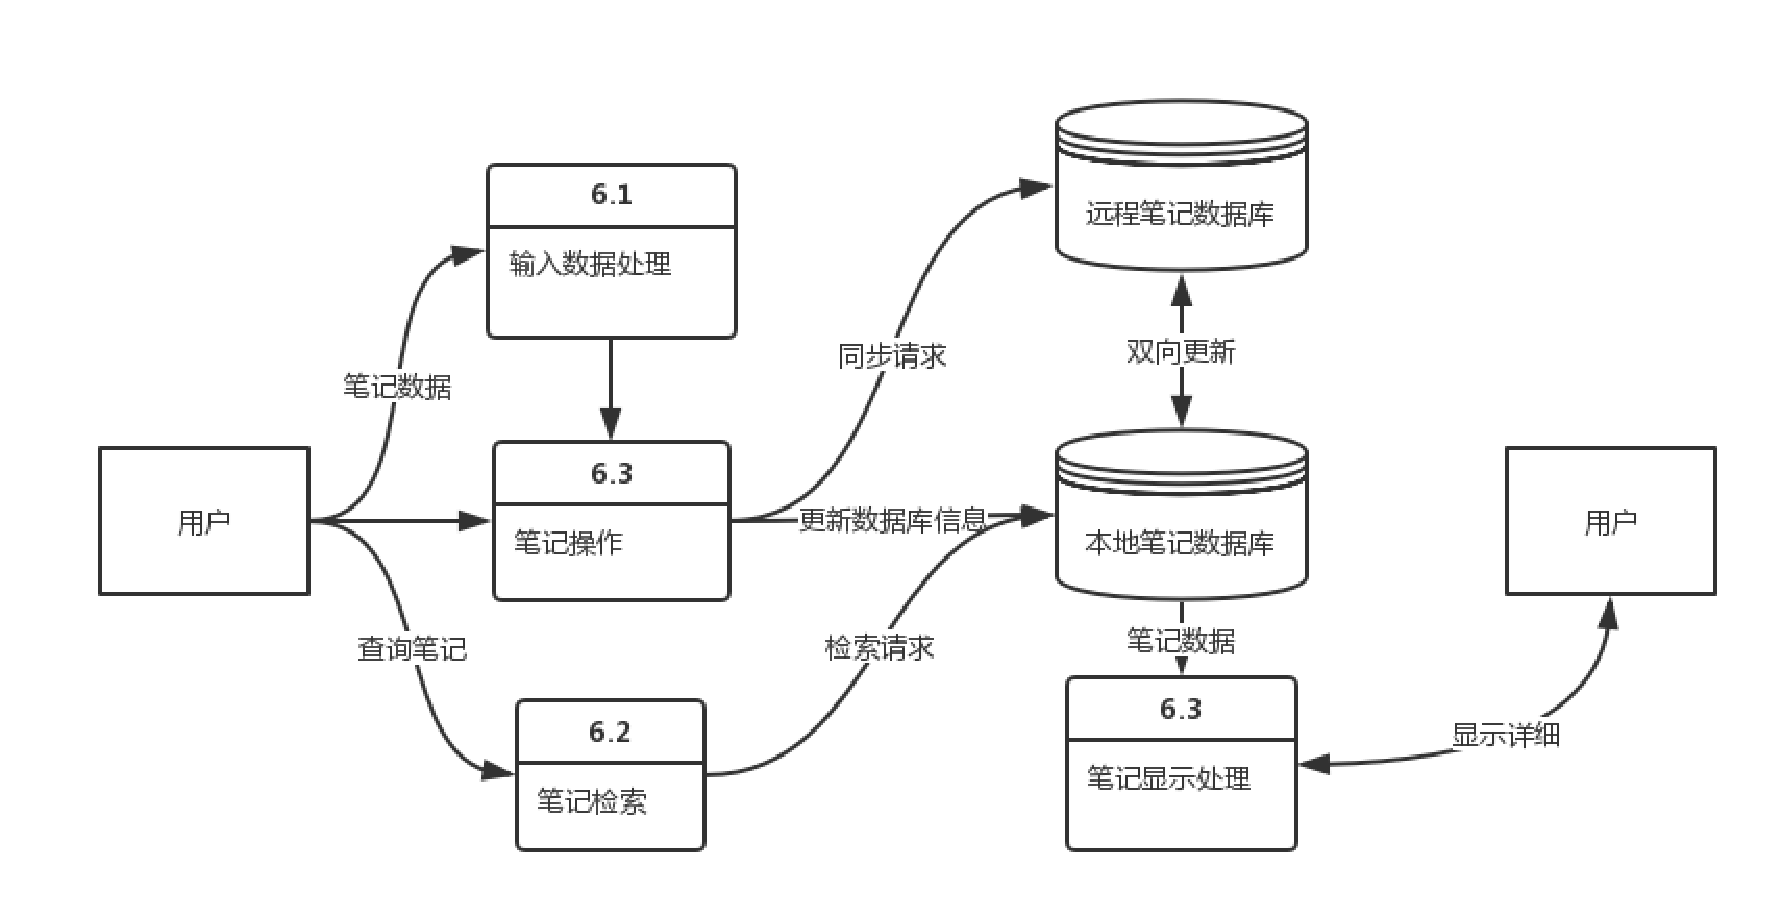
\includegraphics[width=15cm]{level1_学习笔记}
\caption{学习笔记模块功能数据流图}
\end{figure}
\subsubsection{成绩管理模块}
\begin{figure}[H]
\centering
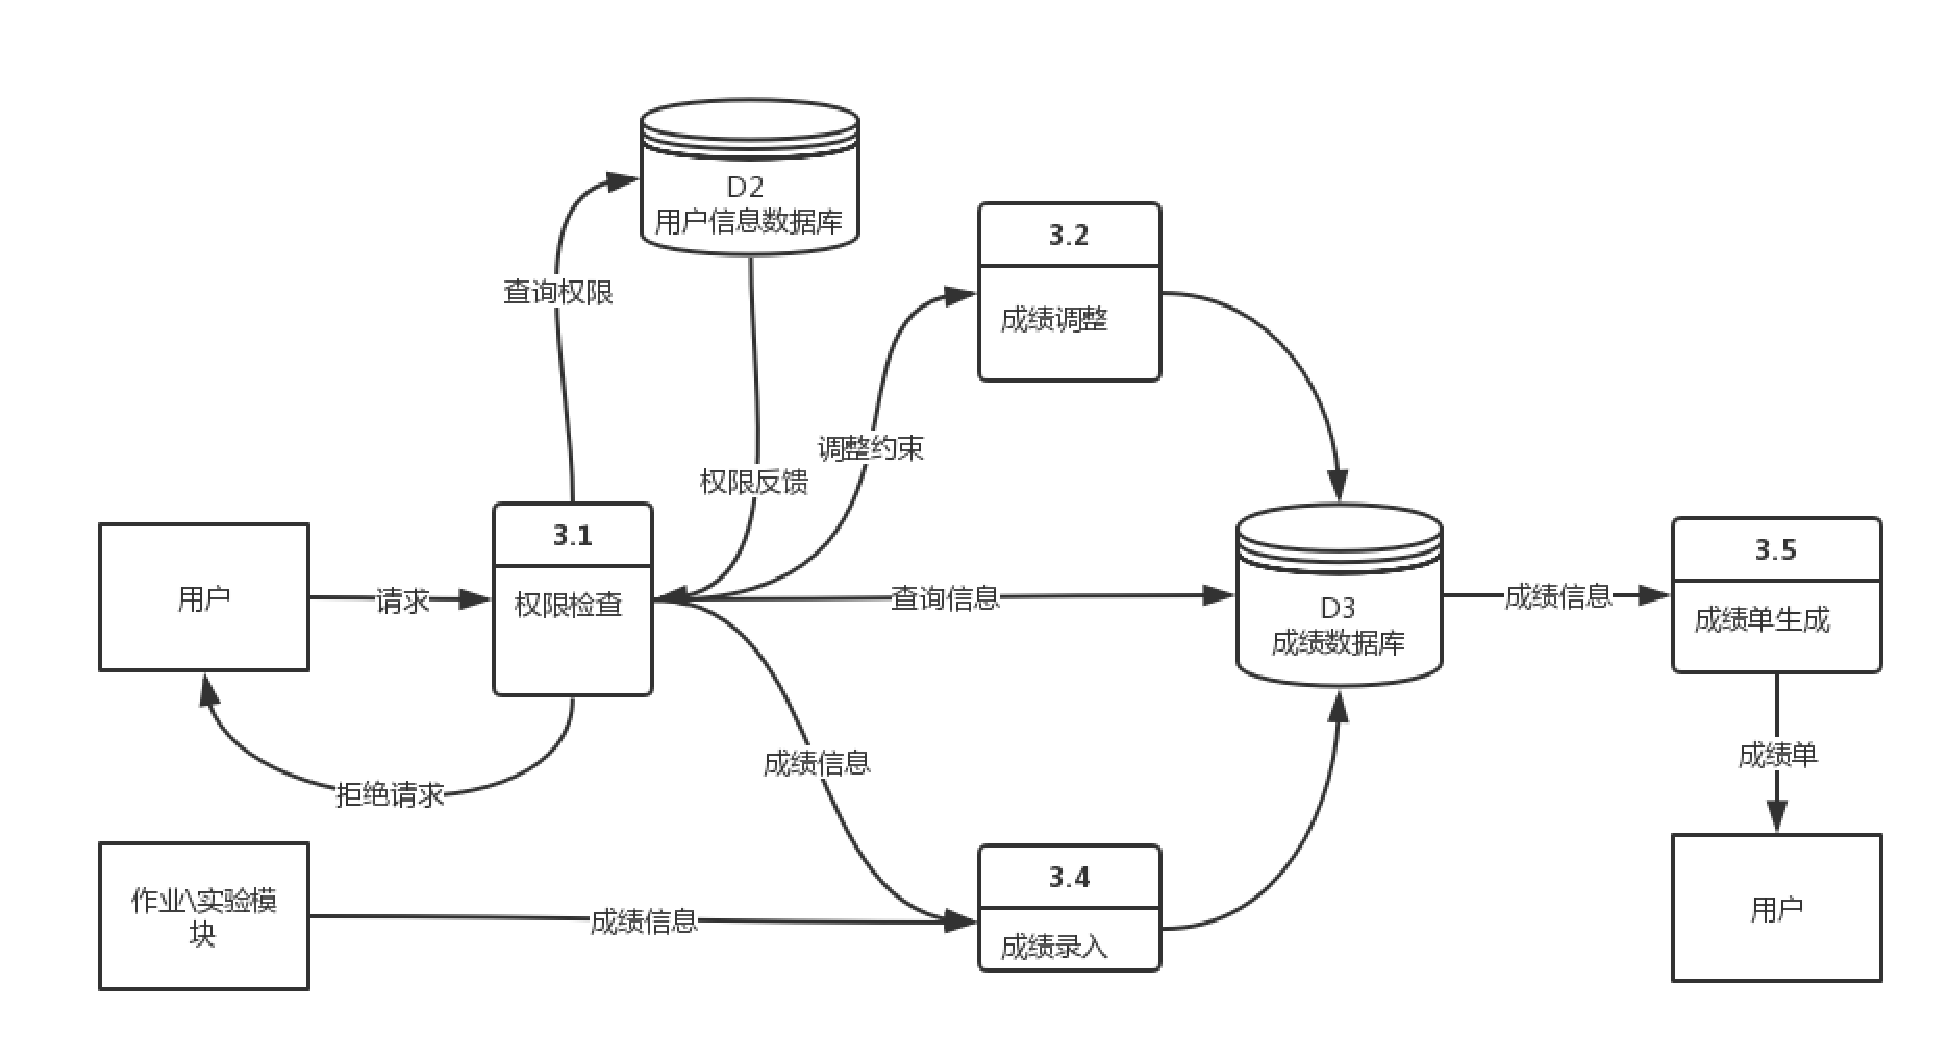
\includegraphics[width=15cm]{level1_成绩管理}
\caption{成绩管理模块功能数据流图}
\end{figure}
\subsubsection{用户管理模块}
\begin{figure}[H]
\centering
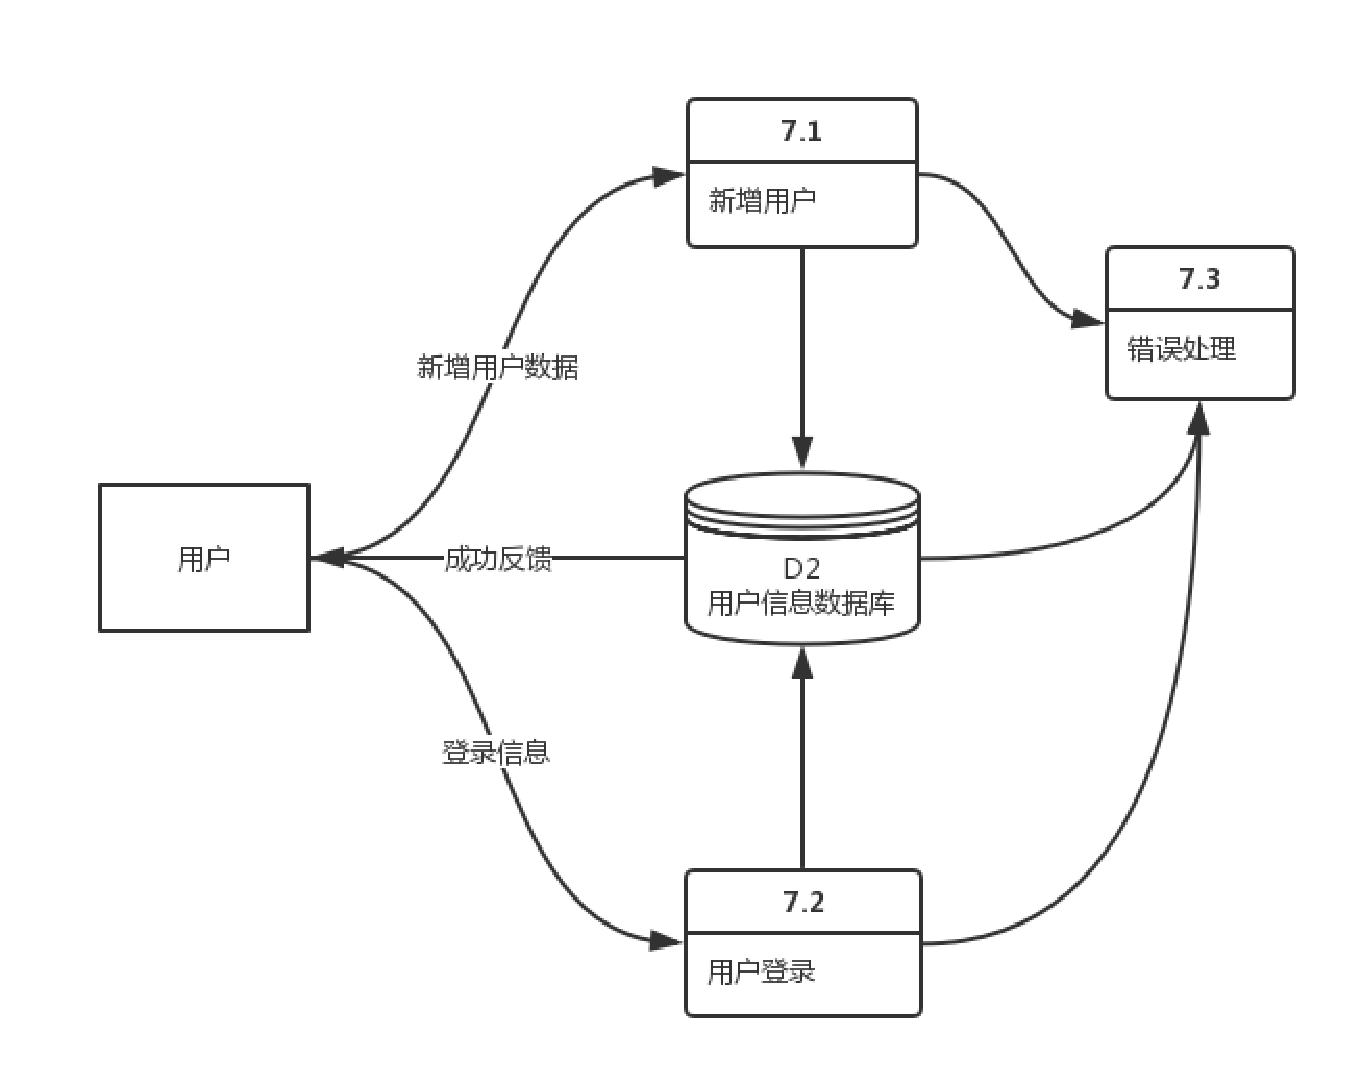
\includegraphics[width=15cm]{level1_用户管理}
\caption{用户理模块功能数据流图}
\end{figure}
\subsubsection{讨论区模块}
\begin{figure}[H]
\centering
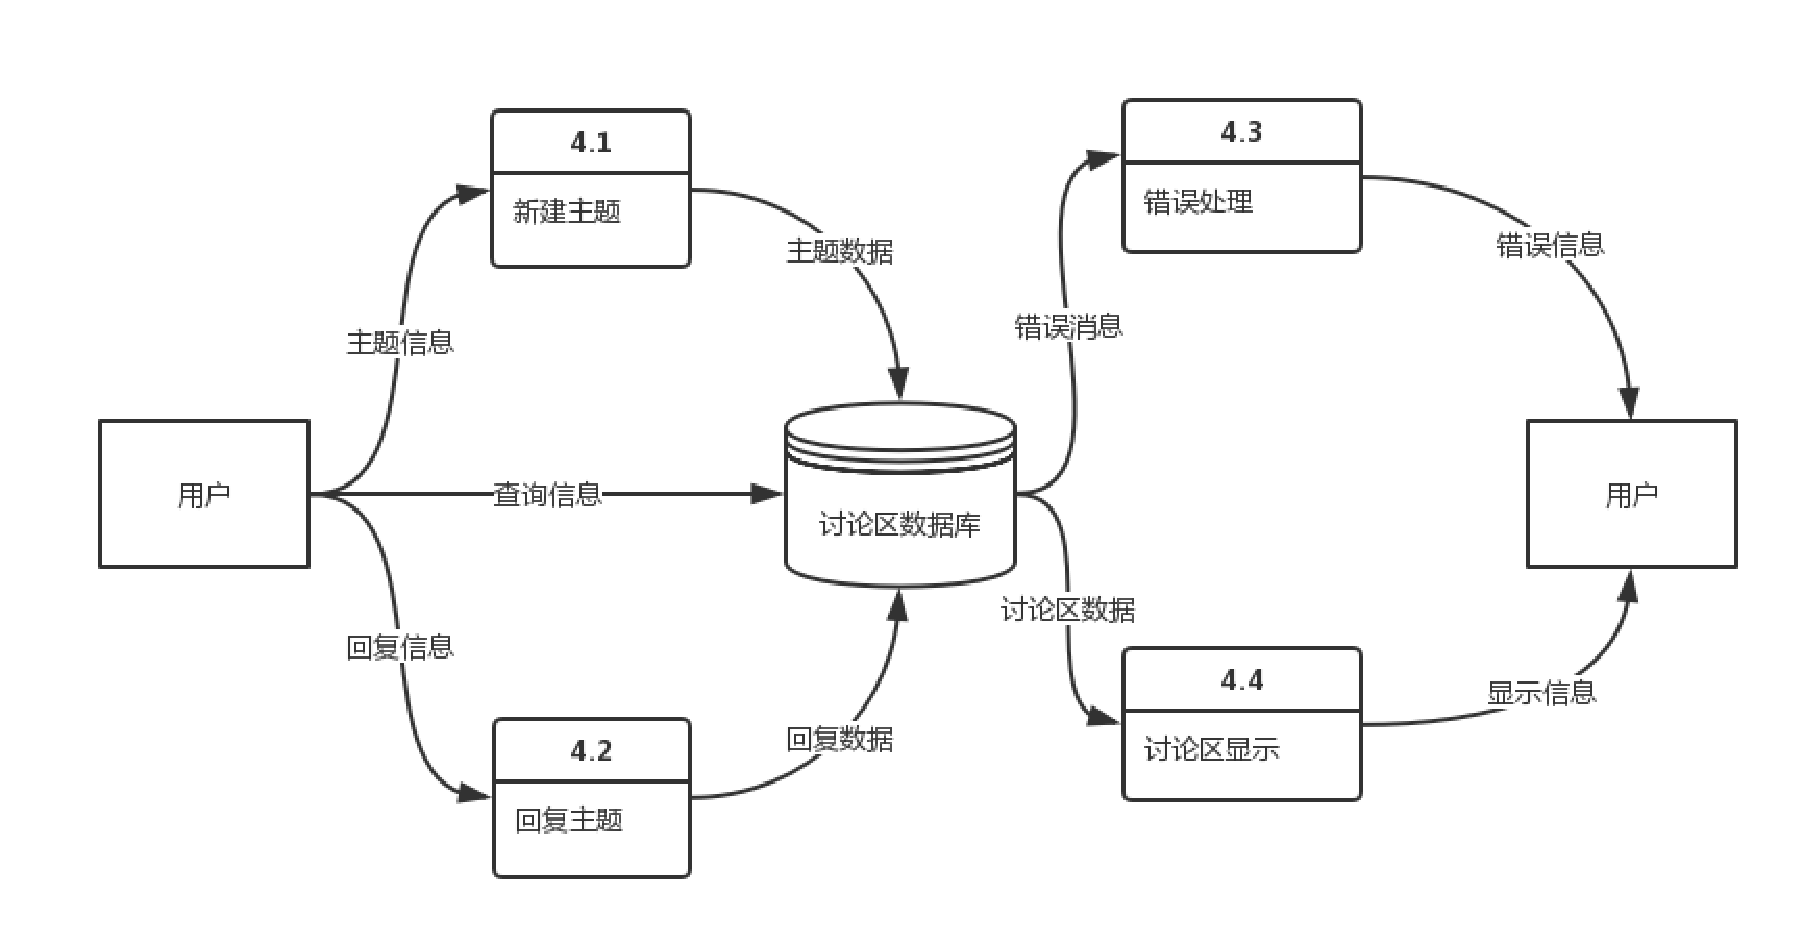
\includegraphics[width=15cm]{level1_讨论区}
\caption{讨论区模块功能数据流图}
\end{figure}
\subsubsection{资源共享模块}
\begin{figure}[H]
\centering
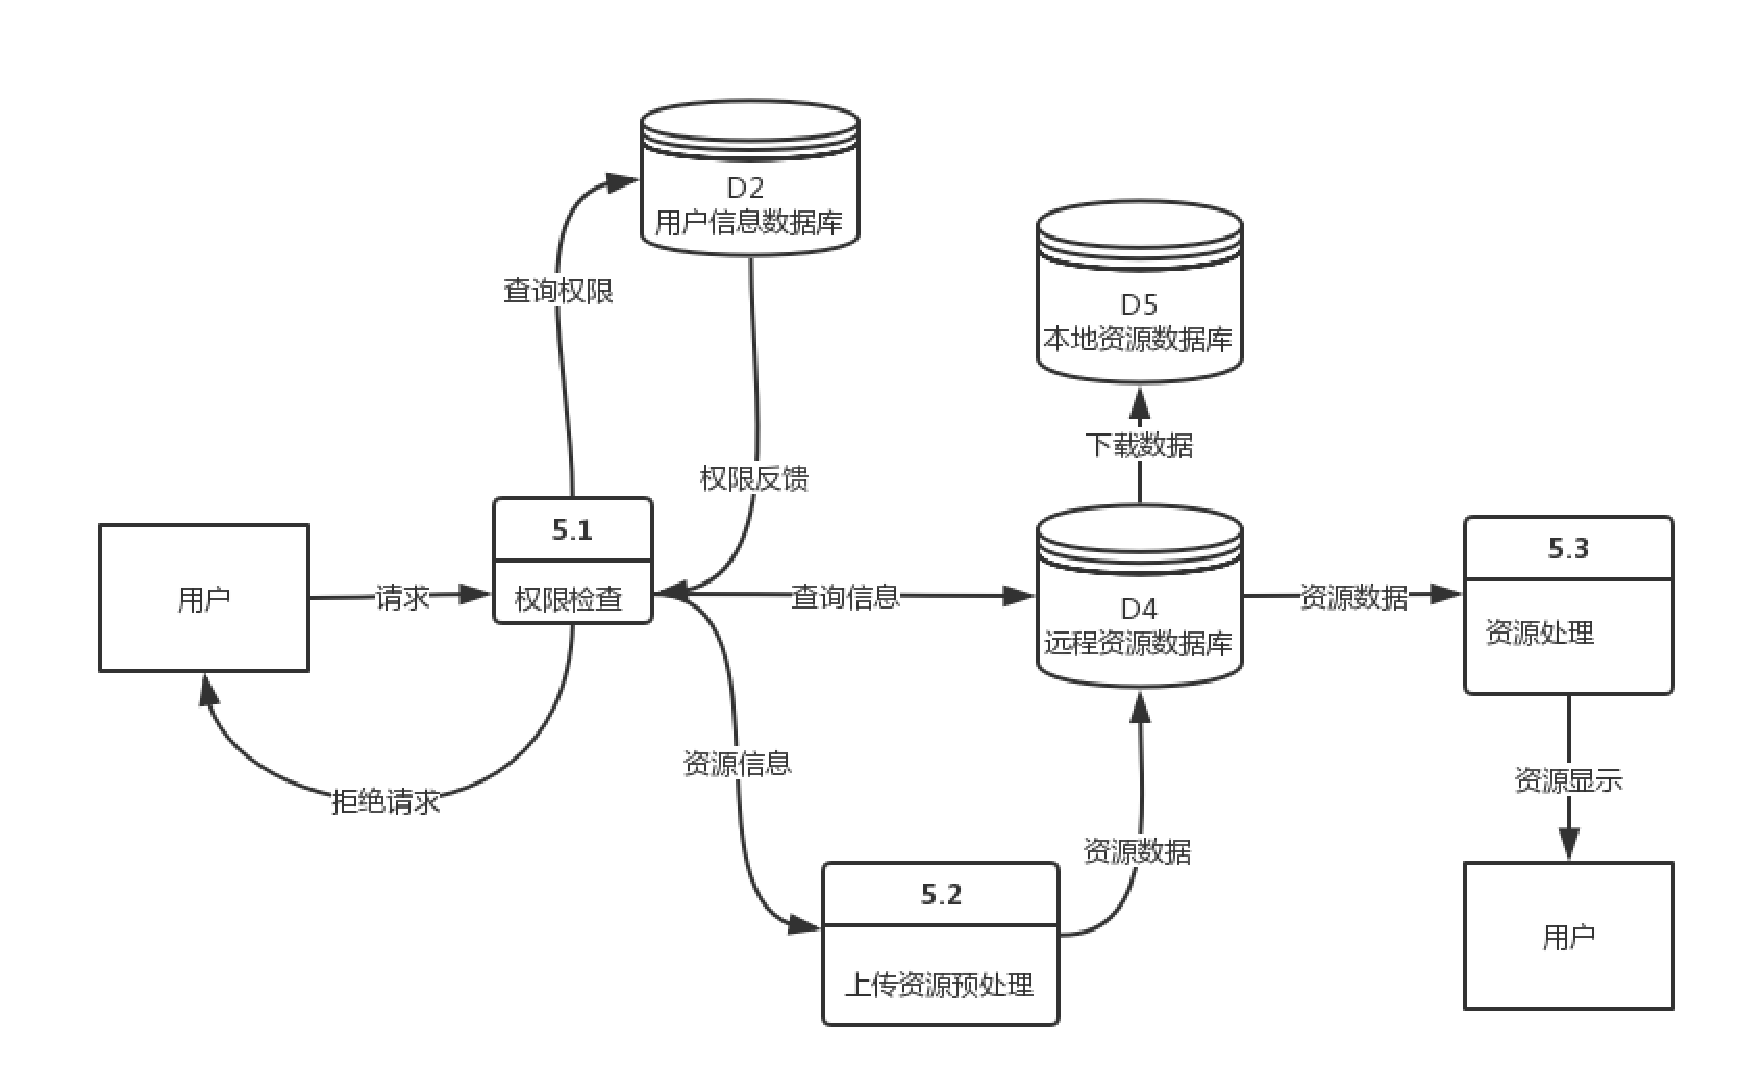
\includegraphics[width=15cm]{level1_资源共享}
\caption{资源共享模块功能数据流图}
\end{figure}
\subsubsection{通知管理模块}
\begin{figure}[H]
\centering
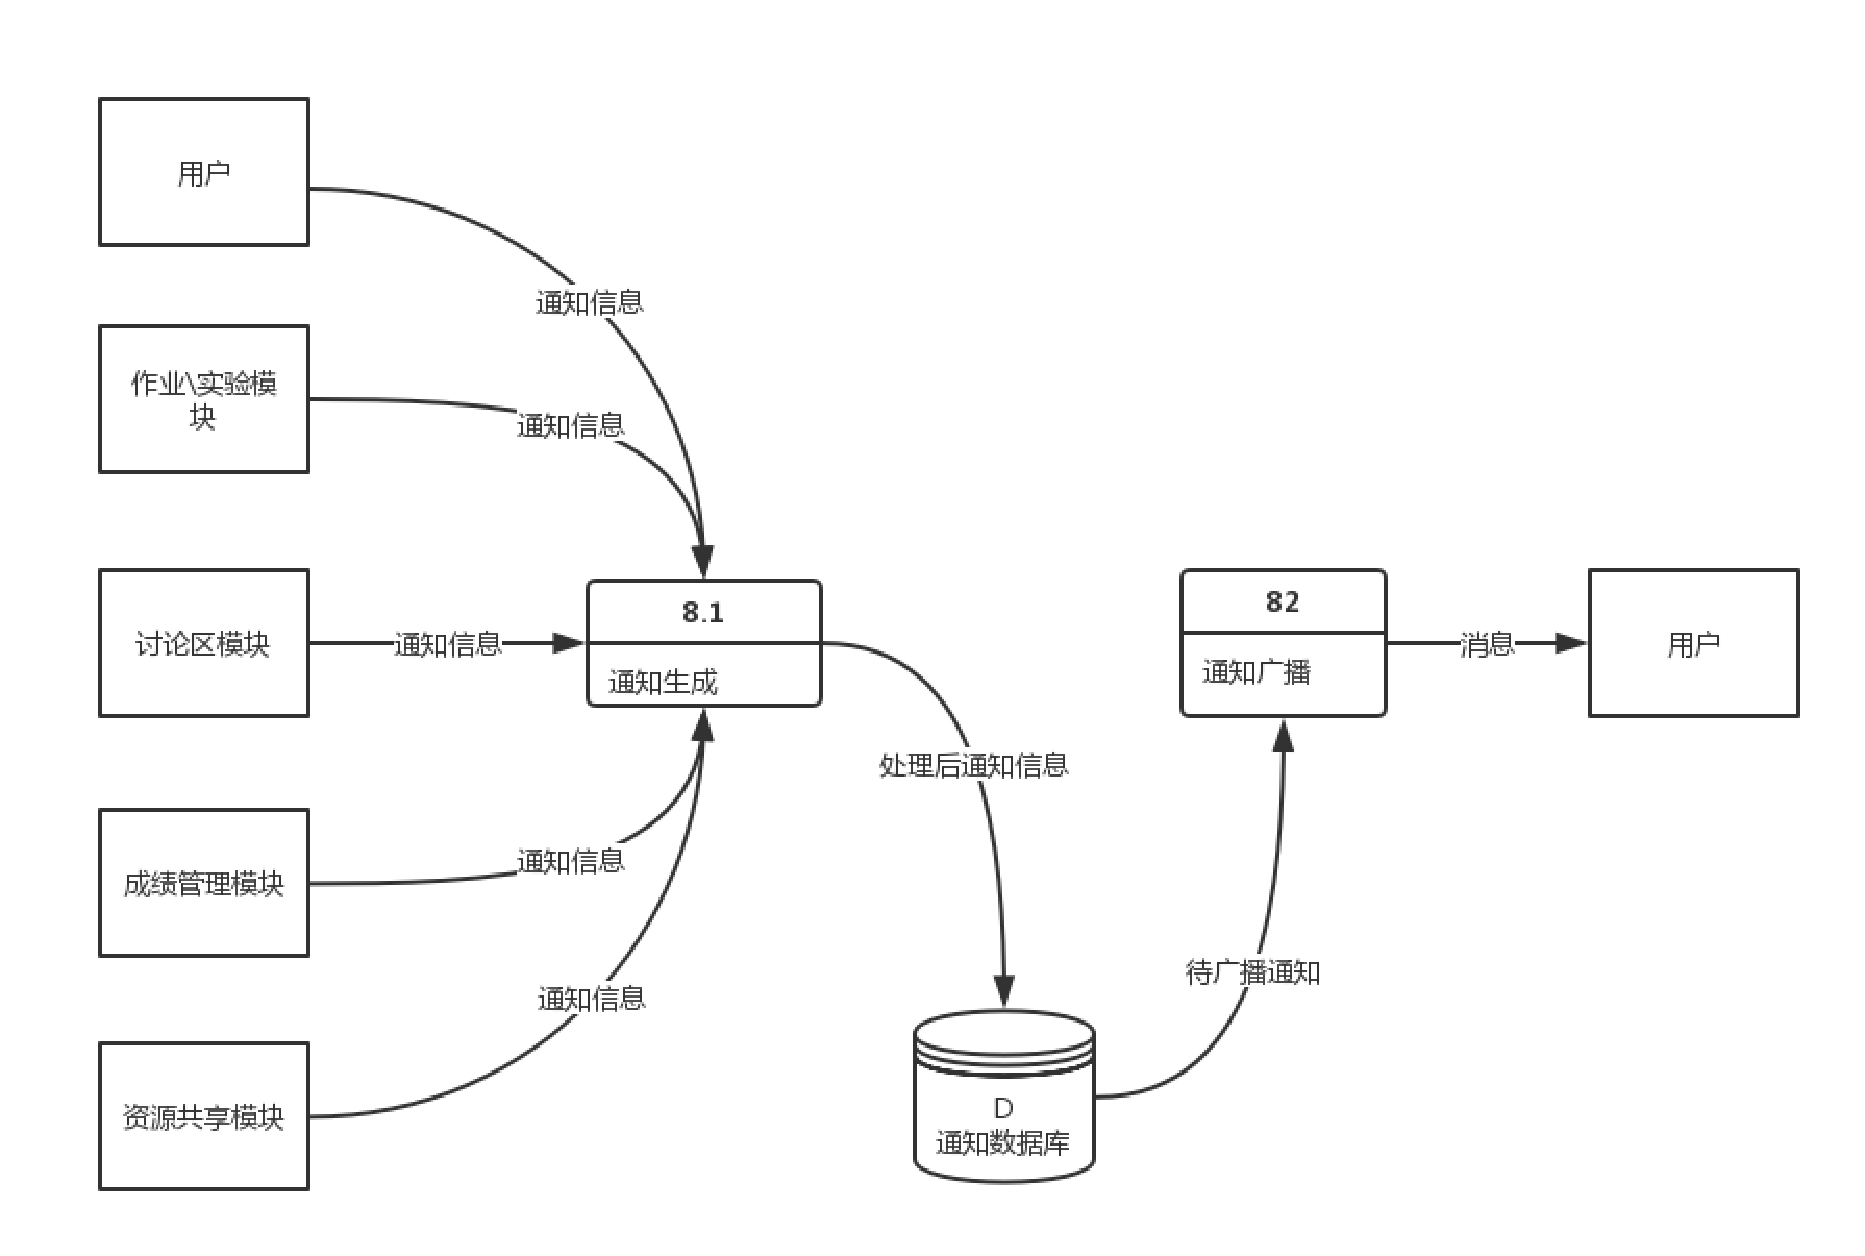
\includegraphics[width=15cm]{level1_通知管理}
\caption{通知管理模块功能数据流图}
\end{figure}

\section{数据字典}
\subsection{数据流说明}
\subsubsection{请求}
来源:用户
简述:用户对数据“请求操作”
去向:请求解析

\subsubsection{信息录入}
来源:请求解析
简介:讲用户信息录入数据库
去向:用户管理模块

\subsubsection{用户信息}
来源:用户管理模块
简介:从数据库中导出的用户信息
去向:返回数据解析

\subsubsection{反馈}
来源:返回数据解析
简介:客户端对于用户数据的处理结果
去向:用户

\subsubsection{笔记创建}
来源:请求解析
简介:新的笔记条目的创建
去向:学习笔记模块

\subsubsection{笔记内容}
来源:学习笔记模块
简介:用户查询的笔记内容
去向:返回数据解析




\subsubsection{笔记数据}
来源:用户,本地笔记数据库
简介:用户的笔记内容
去向:输入数据处理,笔记操作,笔记显示处理

\subsubsection{查询笔记}
来源:用户
简介:对笔记数据进行查询请求
去向:笔记检索

\subsubsection{同步请求}
来源:笔记操作
简述:客户端与远程笔记同步
去向:远程笔记数据库

\subsubsection{更新数据库信息}
来源:笔记操作
简述:向客户端提出更新数据库命令
去向:本地笔记数据库

\subsubsection{双向更新}
来源:远程笔记数据库,本地笔记数据库
简述:客户端与远程笔记双向更新
去向:远程笔记数据库,本地笔记数据库

\subsubsection{检索请求}
来源:笔记检索
简述:在客户端查询笔记
去向:本地笔记数据库

\subsubsection{显示详细}
来源:笔记显示处理
简述:将笔记数据显示到用户界面
去向:用户

\subsubsection{新增用户数据}
来源:用户
简介:在数据库中增加用户
去向:新增用户

\subsubsection{成功反馈}
来源:用户信息数据库
简介:反馈给用户新增数据成功
去向:用户

\subsubsection{登录信息}
来源:用户,用户登录
简介:讲用户的登录信息在用户和客户端间同步
去向:用户,用户登录


\subsection{数据存储说明}
\subsubsection{数据存储1名称}
<Title of  the data flow should accord with the one in data flow diagram, and the Data description notions should be used. The arrangement of the data in data store should also be described.>

与数据流图中的名称一致,采用数据描述符号说明数据流的内容,另外还需描述数据排列方式

\subsubsection{数据存储2名称}
<Title of  the data flow should accord with the one in data flow diagram, and the Data description notions should be used.The arrangement of the data in data store should also be described.>

与数据流图中的名称一致,采用数据描述符号说明数据流的内容,另外还需描述数据排列方式

\subsection{加工说明}
\subsubsection{加工1名称}
<Use natural language, Decision table/Decision tree and Pseudocode to describe how to process the data flow>

采用自然语言,判断表/判断树,伪码的形式描述对数据流进行处理的过程

\subsubsection{加工2名称}
<Use natural language, Decision table/Decision tree and Pseudocode to describe how to process the data flow>

采用自然语言,判断表/判断树,伪码的形式描述对数据流进行处理的过程
